\chapter{Wstęp}
\label{cha:wstęp}

Mimo wynalezienia druku przez Jana Gutenberga w drugiej połowie XV wieku liczba ręcznie spisywanych dokumentów każdego dnia nie spadła aż do wynalezienia maszyny do pisania. Wynikiem tego było gromadzenie ogromnej liczby ręcznie pisanych akt, które obecnie w wielu instytucjach są digitalizowane. Rezultatem są ogromne zbiory danych, często dostępne za darmo w internecie, które jednak nie pozwalają na szybkie znajdowanie potrzebnych informacji ze względu nieustrukturyzowaną formę danych, powodując możliwość wyciągnięcia z nich informacji wyłącznie poprzez czytanie każdej pozycji przez badacza.
Próbą odpowiedzi na ten problem jest niniejsza praca, która swoim zasięgiem obejmuje przegląd obecnych rozwiązań zajmujących się tematyką rozpoznawania pisma odręcznego (ang. HTR – Handwritten Text Recognition) oraz implementację algorytmu odczytującego pismo ręczne.


%---------------------------------------------------------------------------

\section{Problem}
\label{sec:celePracy}


Podstawowym problemem w rozpoznawaniu ręcznego pisma jest indywidualny charakter pisma każdego człowieka. Z tego powodu problem nie był możliwy do rozwiązania za pomocą konwencjonalnych sposobów programowania, ze względu na nieustrukturyzowaną logikę. Oprócz charakteru pisma istotnym elementem jest usytuowanie linii tekstu. Autor, oprócz brzydkiego pisma, może także mieć problem z pisaniem równo, szczególnie na czystych kartkach. Innymi problemami może być słaba jakość dokumentów, zmiana stylu pisania, zakreślania, podkreślenia i zmiana pochyłu pisma.
Założeniem pracy jest obraz wejściowy będący tekstem na czystej kartce, to znaczy bez m.in. kratek, tabel i ilustracji. Pierwotnie praca była motywowana wykorzystaniem jej do pracy nad XIX – wiecznymi dokumentami parafialnymi, tj. księgami urodzin, małżeństw i zgonów, których przykład przedstawiono poniżej (rys. \ref{fig:old}).

\begin{figure}[h!]
    \centering
  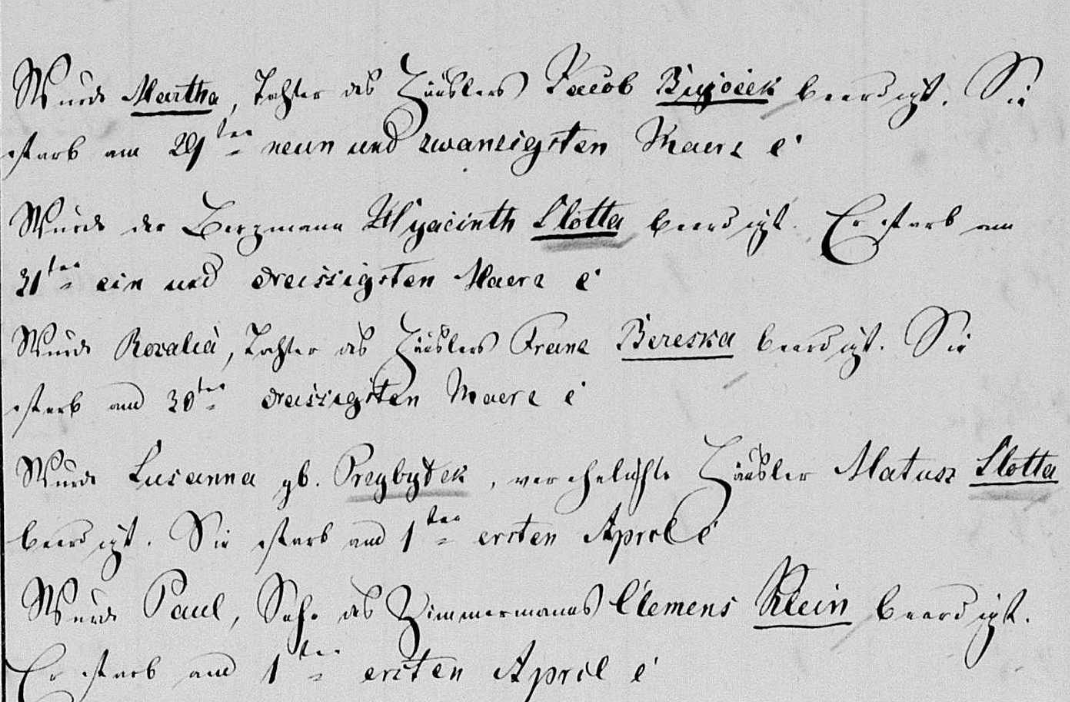
\includegraphics[width=1\textwidth]{2.png}
    \caption{Fragment księgi urodzeń parafii Żyglin na Śląsku, druga połowa XIX wieku.
Źródło familysearch.org}
\label{fig:old}
\end{figure}

Wstępna analiza problemu wykazała, że nie znaleziono odpowiednio dużego zbioru danych, który pozwoliłby na nauczenie modeli sztucznej inteligencji. Z tego powodu za cel pracy przyjęto rozpoznawanie pisma z dostępnego publicznie zbioru danych. Jednak, aby kompletnie nie porzucić pierwotnego problemu, przyjęto architekturę rozwiązania na dwa osobne komponenty:
\begin{itemize}
  \item Podział tekstu na linie;
  \item Rozpoznanie tekstu z linii.
\end{itemize}
Powyższy podział umożliwia przygotowanie rozwiązania, które będzie w stanie przygotować każdy tekst historyczny do uczenia modelu sztucznej inteligencji. 


\subsection{Zbiór danych}

Zbiór danych wykorzystywany w pracy znany jest pod nazwą „IAM Handwriting Database”. Jest to baza danych złożona z 1539 stron tekstu, napisanego przez 657 autorów w języku angielskim. Dokumenty zostały zeskanowane z rozdzielczością 300dpi w skali szarości. Zbiór jest dostępny publicznie [https://fki.tic.heia-fr.ch/databases/iam-handwriting-database] w różnych konfiguracjach:
\begin{itemize}
  \item 1539 stron
  \item 5685 zdań
  \item 13 353 linii
  \item 115 320 słów
\end{itemize}
Każdej wersji odpowiada plik z treścią kolejnych zdjęć. Zbiór, który został wykorzystany jest najpopularniejszym modelem używanym w tego typu programach, co pozwala na szerokie porównanie wyników jego działania do innych prac w tej tematyce.
Baza jest dobrze zbalansowana, znajdują się w niej teksty o różnej wielkości, grubości, pochyleniu. Zaznaczyć należy, że nie linie tekstu są zazwyczaj stosunkowo proste.
Na poniższej ilustracji przedstawiono przykładową stronę ze zbioru IAM Dataset (rys. \ref{fig:IAMexample}).

\begin{figure}[h!]
    \centering
  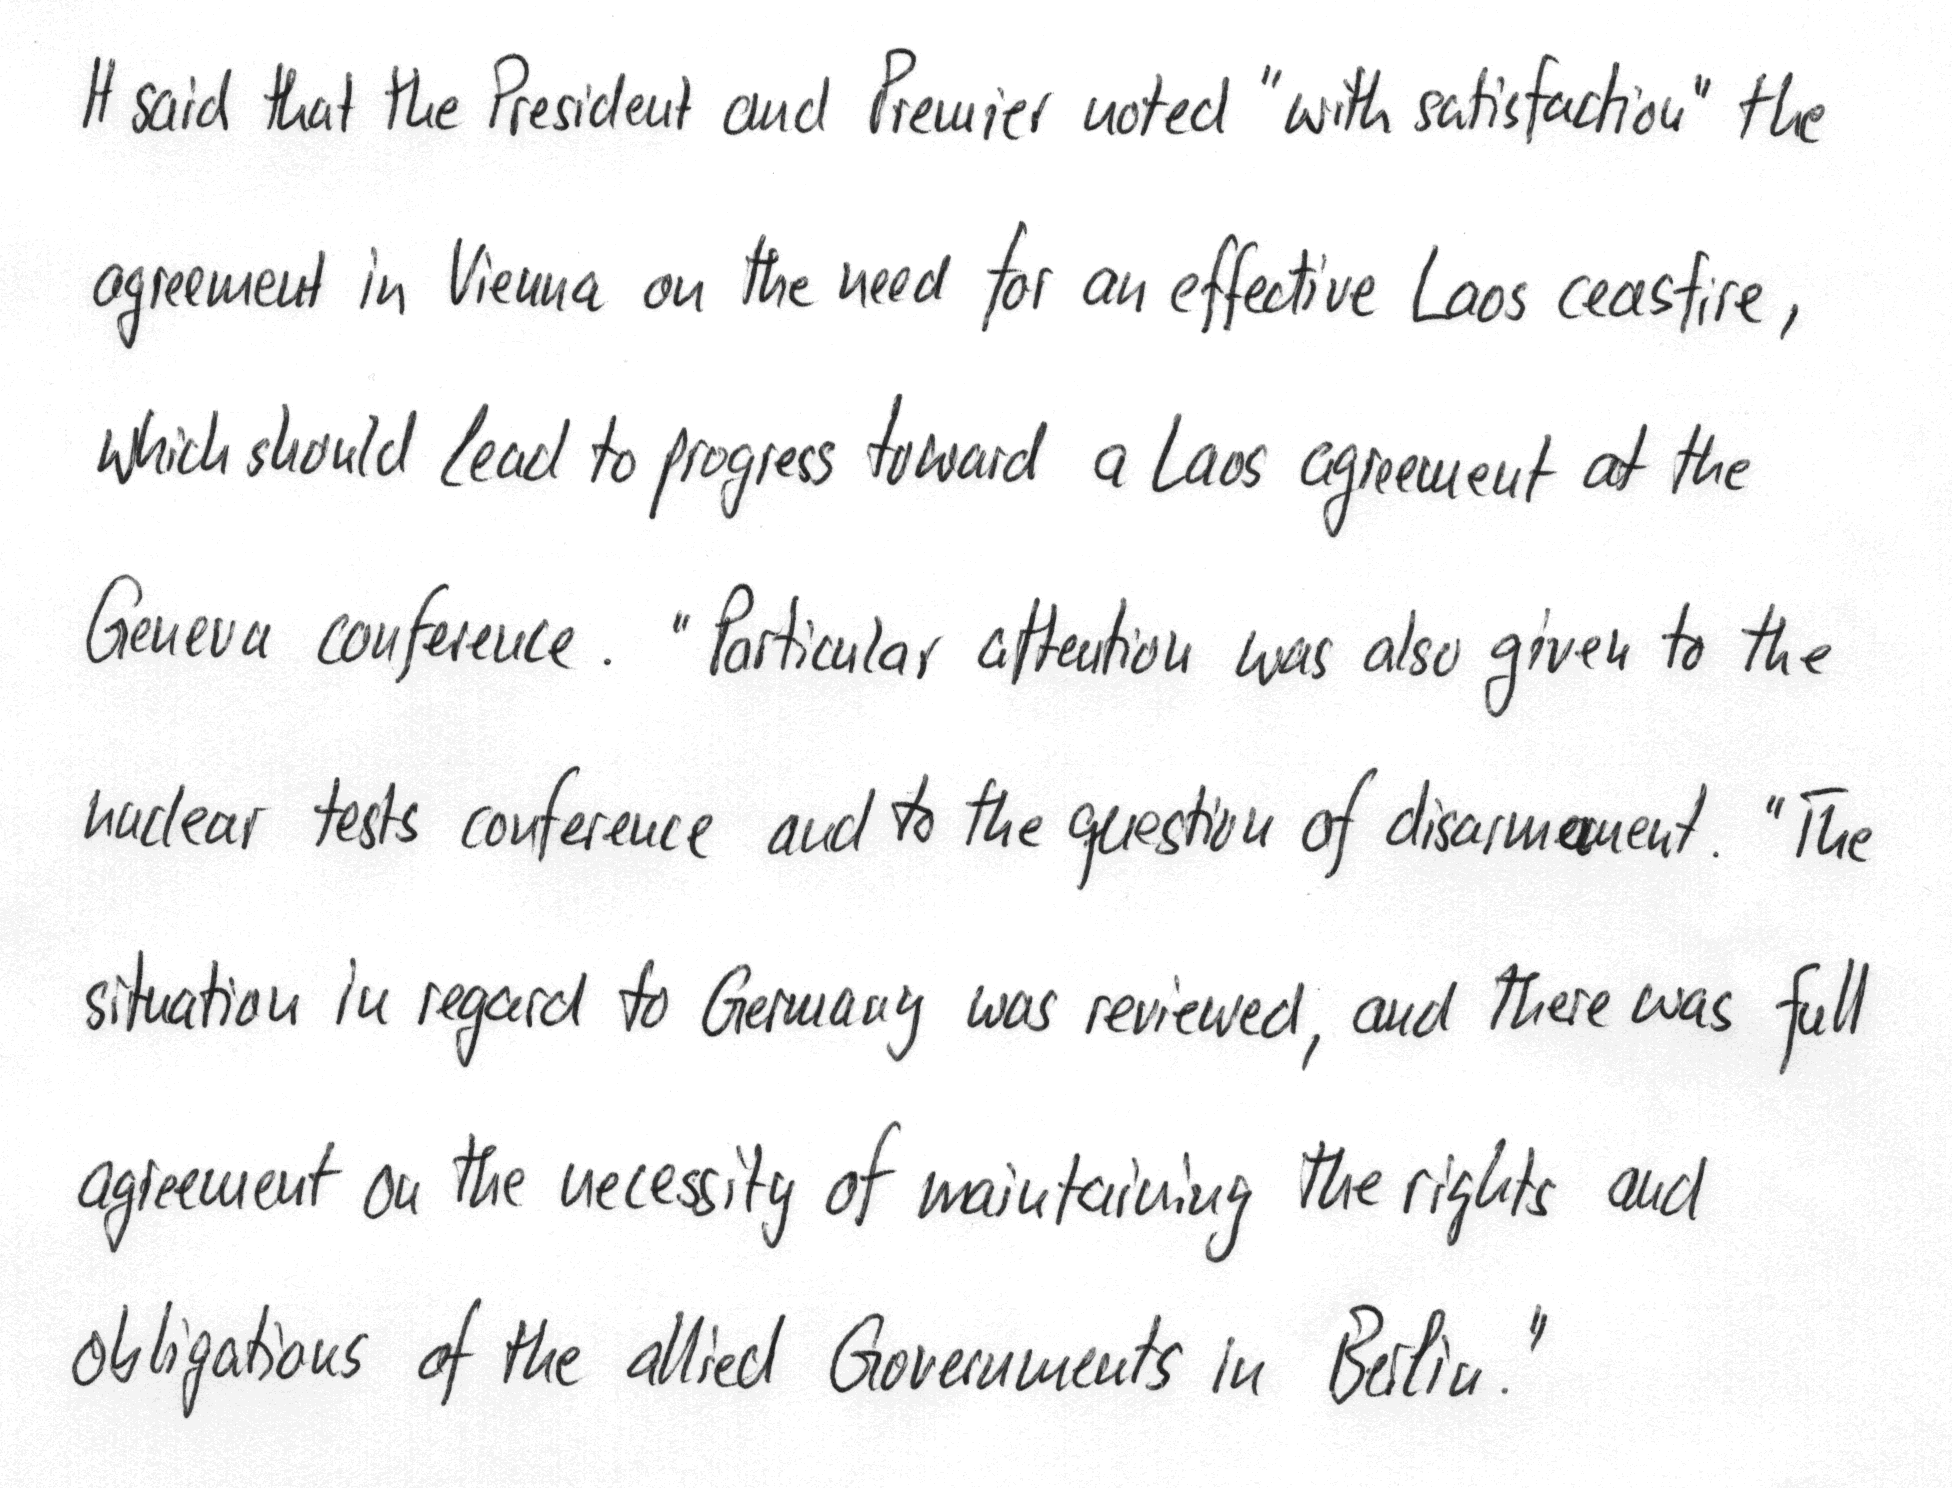
\includegraphics[width=1\textwidth]{przykladIAM.png}
    \caption{Przykładowa strona czystego tekstu z IAM dataset}
\label{fig:IAMexample}
\end{figure}



\subsubsection{Jakiś tytuł w subsubsection}


\subsection{Jakiś tytuł 2}

%---------------------------------------------------------------------------

\section{Zawartość pracy}
\label{sec:zawartoscPracy}

W rodziale~\ref{cha:pierwszyDokument} przedstawiono podstawowe informacje dotyczące struktury dokumentów w \LaTeX u. Alvis~\cite{Alvis2011} jest językiem 


















